\documentclass[12pt, a4paper]{article}
\usepackage[a4paper,top=1.5cm, bottom=1.5cm, left=2cm, right=2cm]{geometry}
\usepackage{graphicx} % Required for inserting images
%%% Работа с русским языком
\usepackage{cmap}					% поиск в PDF
\usepackage{mathtext} 				% русские буквы в фомулах
\usepackage[T2A]{fontenc}			% кодировка
\usepackage[utf8]{inputenc}			% кодировка исходного текста
\usepackage[english,russian]{babel}	% локализация и переносы
\usepackage{float}
\usepackage{subcaption}
\usepackage{wrapfig}
\usepackage{tabularx}
\usepackage{multirow}

\usepackage[unicode, colorlinks=true, urlcolor=blue]{hyperref}
\usepackage[rgb]{xcolor}
\hypersetup{
colorlinks=true,urlcolor=blue
}
%%% Дополнительная работа с математикой
\usepackage{amsmath,amsfonts,amssymb,amsthm,mathtools} % AMS
\usepackage{icomma} % "Умная" запятая: $0,2$ --- число, $0, 2$ --- перечисление
%% Номера формул
\mathtoolsset{showonlyrefs=true} % Показывать номера только у тех формул, на которые есть \eqref{} в тексте.
%% Шрифты
\usepackage{euscript}	 % Шрифт Евклид
\usepackage{mathrsfs} % Красивый матшрифт
%% Свои команды
\DeclareMathOperator{\sgn}{\mathop{sgn}}
%% Перенос знаков в формулах (по Львовскому)
\newcommand*{\hm}[1]{#1\nobreak\discretionary{}
{\hbox{$\mathsurround=0pt #1$}}{}}


\usepackage{indentfirst}
\usepackage{amsmath,amssymb}
\usepackage[italicdiff]{physics}
\graphicspath{{images/}}
\DeclareGraphicsExtensions{.pdf,.png,.jpg}
\usepackage{enumitem}
\usepackage{caption}
\usepackage{array}
\usepackage{ragged2e}







\begin{document}



\include{titlepage}
\begin{titlepage}
\thispagestyle{empty}

\begin{center}
\small
Министерство науки и высшего образования Российской Федерации\\[2mm]
\textbf{ФЕДЕРАЛЬНОЕ ГОСУДАРСТВЕННОЕ АВТОНОМНОЕ
ОБРАЗОВАТЕЛЬНОЕ УЧРЕЖДЕНИЕ ВЫСШЕГО ОБРАЗОВАНИЯ}\\[1mm]
«МОСКОВСКИЙ ФИЗИКО-ТЕХНИЧЕСКИЙ ИНСТИТУТ\\
(НАЦИОНАЛЬНЫЙ ИССЛЕДОВАТЕЛЬСКИЙ УНИВЕРСИТЕТ)»\\
(МФТИ, Физтех)
\end{center}

\vspace{18mm}

\begin{center}
\large \textbf{КАФЕДРА ЭЛЕКТРОНИКИ}\\[10mm]
\Large \textbf{ОТЧЁТ}\\[2mm]
\large \textbf{ПО ЛАБОРАТОРНОЙ РАБОТЕ}\\[14mm]
\Large \textbf{АТОМНО-СИЛОВОЙ МИКРОСКОП}
\end{center}

\vfill

% Блоки с подписями слева, линии и пояснения справа
\noindent
\begin{tabular}{@{}p{0.44\linewidth}p{0.52\linewidth}@{}}
\textit{Работу выполнили:} & Рагозина Елизавета,

Струков Олег,

Топольский Михаил,

Группа Б04-404 \\[8mm]

\textit{Работу принял, оценка:} & \\[3mm]
 \\
\end{tabular}


\vspace{12mm}

\begin{center}
\small Долгопрудный, \the\year{}~г.
\end{center}

\end{titlepage}




\newpage
\pagenumbering{arabic}


\section{Теоретическая часть}

\subsection{Физические принципы атомно-силовой микроскопии}

Атомно-силовой микроскоп (АСМ) --- прибор для исследования топографии поверхности с нанометровым разрешением, основанный на регистрации сил взаимодействия между острым зондом и образцом. В отличие от сканирующего туннельного микроскопа, АСМ позволяет изучать как проводящие, так и непроводящие материалы.

При сканировании на воздухе основной вклад в силовое взаимодействие вносят:
\begin{itemize}
    \item силы Ван-дер-Ваальса (дальнодействующее притяжение);
    \item капиллярные силы (притяжение из-за плёнки адсорбированной воды);
    \item силы отталкивания (при непосредственном контакте электронных оболочек).
\end{itemize}

Зависимость силы взаимодействия $F$ от расстояния $z$ между зондом и образцом показана на рис.~\ref{fig:force_distance}. Различают три режима работы АСМ в зависимости от рабочей точки на этой кривой:
\begin{enumerate}
    \item \textbf{Контактный режим} --- зонд находится в области отталкивания ($F > 0$);
    \item \textbf{Полуконтактный режим} --- зонд колеблется, периодически касаясь поверхности;
    \item \textbf{Бесконтактный режим} --- зонд колеблется в области притяжения ($F < 0$), не касаясь поверхности.
\end{enumerate}

\begin{figure}[h!]
    \centering
    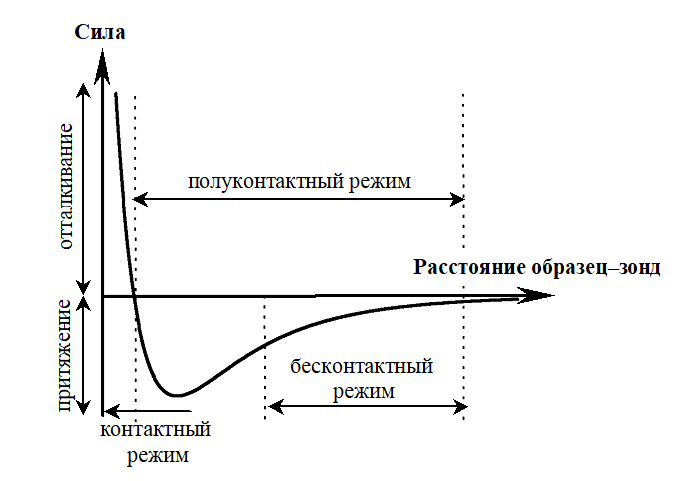
\includegraphics[width=0.6\textwidth]{1.png}
    \caption{Зависимость силы взаимодействия зонда с поверхностью от расстояния. Области соответствуют различным режимам работы АСМ.}
    \label{fig:force_distance}
\end{figure}

\subsection{Устройство сканирующего зондового микроскопа NanoEducator}

Основными элементами АСМ являются: зонд (кантилевер с остриём), пьезосканер, система регистрации отклонений и система обратной связи.

В приборе \textit{NanoEducator} используется оригинальная конструкция датчика силового взаимодействия на основе пьезокерамической трубки (рис.~\ref{fig:piezo_tube}). Трубка длиной $l = 7$~мм, диаметром $d = 1{,}2$~мм и толщиной стенки $h = 0{,}25$~мм жёстко закреплена с одного конца. На внутреннюю поверхность нанесён проводящий электрод, на внешнюю --- два электрически изолированных полуцилиндрических электрода. К свободному концу прикреплена вольфрамовая проволока диаметром $100$~мкм, заточенная электрохимически (радиус закругления острия $0{,}05$--$0{,}2$~мкм).

\begin{figure}[h!]
    \centering
    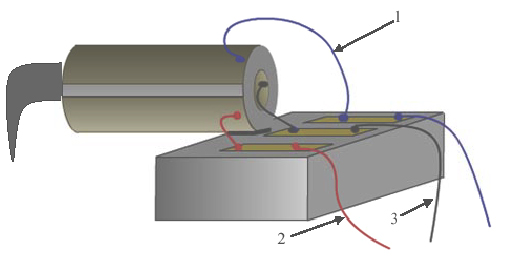
\includegraphics[width=0.5\textwidth]{2.png}
    \caption{Конструкция датчика силового взаимодействия NanoEducator: (1) провод генератора; (2) провод датчика; (3) общий провод.}
    \label{fig:piezo_tube}
\end{figure}

Одна часть пьезотрубки работает как пьезовибратор (возбуждает колебания зонда), другая --- как датчик механических колебаний (регистрирует отклик). При колебаниях зонда на датчике возникает переменное напряжение, пропорциональное смещению.

Пьезосканер перемещает образец по трём координатам $X$, $Y$, $Z$. Он изготовлен из пьезоэлектрического материала (цирконат-титанат свинца), который деформируется пропорционально приложенному напряжению. Основные недостатки пьезокерамики --- нелинейность, гистерезис, ползучесть и температурный дрейф --- требуют учёта при обработке результатов.

\subsection{Бесконтактный режим работы}

В данной работе измерения проводятся в бесконтактном режиме. Кантилевер возбуждается на резонансной частоте $\omega_0$:
\begin{equation}
    \omega_0 = \sqrt{\frac{k}{m}},
    \label{eq:resonance}
\end{equation}
где $k$ --- жёсткость кантилевера, $m$ --- эффективная масса.

Уравнение движения зонда при малой амплитуде колебаний:
\begin{equation}
    m\ddot{z} + \frac{m\omega_0}{Q}\dot{z} + kz = k\Delta z \sin(\omega t) + F(z),
    \label{eq:motion}
\end{equation}
где $Q$ --- добротность колебательной системы, $\Delta z$ --- амплитуда возбуждения, $F(z)$ --- сила взаимодействия зонда с образцом.

Стационарное решение имеет вид:
\begin{equation}
    z(t) = A \sin(\omega t + \varphi),
    \label{eq:stationary}
\end{equation}
где амплитуда $A$ и сдвиг фазы $\varphi$ определяются выражениями:
\begin{equation}
    A = \frac{\Delta z}{\sqrt{\left(1 - \frac{\omega^2}{\omega_0^2}\right)^2 + \left(\frac{\omega}{Q\omega_0}\right)^2}},
    \label{eq:amplitude}
\end{equation}
\begin{equation}
    \tan\varphi = \frac{\frac{\omega}{Q\omega_0}}{1 - \frac{\omega^2}{\omega_0^2}}.
    \label{eq:phase}
\end{equation}

При приближении зонда к поверхности возникает градиент силы $\partial F/\partial z$, что приводит к смещению резонансной частоты:
\begin{equation}
    \omega = \omega_0 \sqrt{1 - \frac{1}{k}\frac{\partial F}{\partial z}}.
    \label{eq:frequency_shift}
\end{equation}

Поскольку частота возбуждения поддерживается равной $\omega_0$, изменение резонансной частоты приводит к изменению амплитуды колебаний. Система обратной связи поддерживает амплитуду постоянной, изменяя расстояние $Z$ между зондом и образцом. Сигнал с $Z$-пьезоэлемента используется для построения топографии.

\subsection{Оценка радиуса закругления зонда}

Латеральное разрешение АСМ ограничено радиусом кривизны острия $R$. При сканировании выступа высотой $\Delta Z$ и шириной $d$ (рис.~\ref{fig:tip_geometry}) зонд не может полностью проникнуть в углубление из-за конечного радиуса закругления.

\begin{figure}[h!]
    \centering
    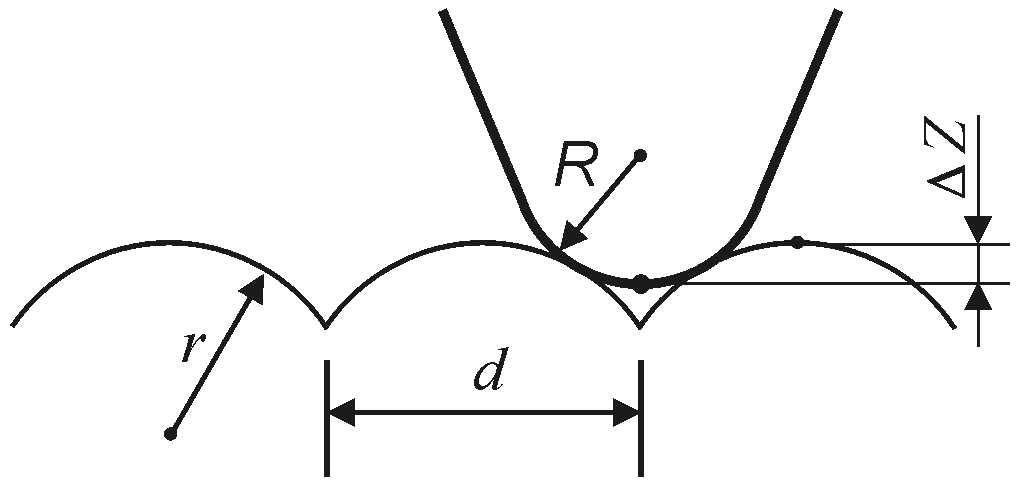
\includegraphics[width=0.5\textwidth]{3.png}
    \caption{Геометрия взаимодействия зонда с выступом: $R$ --- радиус закругления острия, $d$ --- ширина выступа на сечении, $\Delta Z$ --- высота выступа.}
    \label{fig:tip_geometry}
\end{figure}

Из геометрических соображений минимальное расстояние между разрешаемыми объектами (при $r \to 0$):
\begin{equation}
    d = \sqrt{2R\Delta Z}.
    \label{eq:resolution}
\end{equation}

Отсюда радиус закругления зонда оценивается по формуле:
\begin{equation}
    R = \frac{d^2}{2\Delta Z}.
    \label{eq:tip_radius}
\end{equation}

Для калибровки используется тестовая решётка TGT01 с известным периодом $2{,}12$~мкм и радиусом закругления острия порядка $10$~нм.


\subsection{Особенности конструкции NanoEducator}
В используемом в работе микроскопе \textit{NanoEducator} в качестве датчика силового взаимодействия применяется пьезокерамическая трубка длиной $l = 7$~мм, диаметром $d = 1,2$~мм и толщиной стенки $h = 0,25$~мм. К её свободному концу прикреплена вольфрамовая проволока диаметром $100$~мкм, заточенная электрохимически. 

Оригинальность конструкции заключается в том, что одна часть трубки работает как пьезовибратор (возбуждает колебания зонда), а другая --- как тензодатчик, регистрирующий механические колебания. Это позволяет отказаться от громоздкой оптической системы регистрации, характерной для классических АСМ.

\subsection{Искажения пьезосканера}
Перемещение образца осуществляется пьезосканером. Пьезокерамика обладает рядом неидеальностей, которые необходимо учитывать:
\begin{enumerate}
    \item \textbf{Гистерезис} --- неоднозначная зависимость удлинения от направления изменения напряжения. Величина гистерезиса обычно составляет около $10\,\%$.
    \item \textbf{Ползучесть (creep)} --- медленный дрейф положения после быстрого изменения напряжения. Для борьбы с этим эффектом в алгоритмах управления исключают резкие скачки напряжения и вводят временные задержки.
    \item \textbf{Температурный дрейф}. При изменении температуры на $\Delta T = 1^\circ$C пьезотрубка длиной $l = 20$~мм с коэффициентом линейного расширения $\beta = 2 \cdot 10^{-6}$~К$^{-1}$ изменит длину на $\Delta l = \beta l \Delta T = 40$~\AA. Поэтому измерения следует проводить после термостабилизации прибора.
\end{enumerate}

\subsection{Система обратной связи в бесконтактном режиме}
В бесконтактном режиме зонд колеблется на резонансной частоте $\omega_0$ с амплитудой, меньшей зазора между зондом и образцом. При приближении к поверхности возникает градиент силы Ван-дер-Ваальса $\partial F/\partial z$, что приводит к сдвигу резонансной частоты:
\begin{equation}
    \omega = \omega_0 \sqrt{1 - \frac{1}{k}\frac{\partial F}{\partial z}},
\end{equation}
где $k$ --- жёсткость кантилевера. 

Поскольку частота возбуждения фиксирована ($\omega = \omega_0$), изменение резонансной частоты вызывает падение амплитуды колебаний. Система обратной связи (ОС) непрерывно подстраивает напряжение на $Z$-пьезоэлементе так, чтобы амплитуда колебаний оставалась равной заданному значению (Setpoint, $SP$). Массив напряжений, подаваемых на $Z$-электрод, и представляет собой топографию поверхности $Z(x, y)$.

\subsection{Разрешающая способность АСМ}
Вертикальное разрешение АСМ составляет доли ангстрема и ограничено тепловыми шумами. Латеральное (горизонтальное) разрешение ограничено конечным радиусом кривизны острия зонда $R$. 

При сканировании выступа высотой $\Delta Z$ зонд не может полностью проникнуть в узкие углубления. Из геометрических соображений (рис.~\ref{fig:tip_geometry}) минимальное расстояние $d$ между двумя разрешаемыми объектами (или ширина выступа на полученном изображении) связано с радиусом острия соотношением:
\begin{equation}
    d = \sqrt{2R\Delta Z}.
\end{equation}
Эта формула является рабочей для оценки радиуса закругления зонда $R$ по известным геометрическим параметрам калибровочной решётки (высоте $\Delta Z$ и измеренной ширине $d$).





\section*{Ход работы и результаты измерений}

\subsection*{Настройка резонансной частоты зонда}

Перед началом сканирования была снята амплитудно-частотная характеристика (АЧХ) зонда, необходимая для определения рабочей частоты в бесконтактном режиме. Напряжение раскачки зонда было установлено на уровне $12$~мВ, усиление амплитуды --- $2$.

По полученной АЧХ (рис.~\ref{fig:ach}) были определены следующие параметры:
\begin{itemize}
    \item резонансная частота зонда: $f_0 \approx 8{,}8$~кГц;
    \item амплитуда колебаний на резонансе: $A_0 = 1{,}44$~В;
    \item добротность колебательной системы: $Q = 27{,}1$.
\end{itemize}

\begin{figure}[h!]
    \centering
    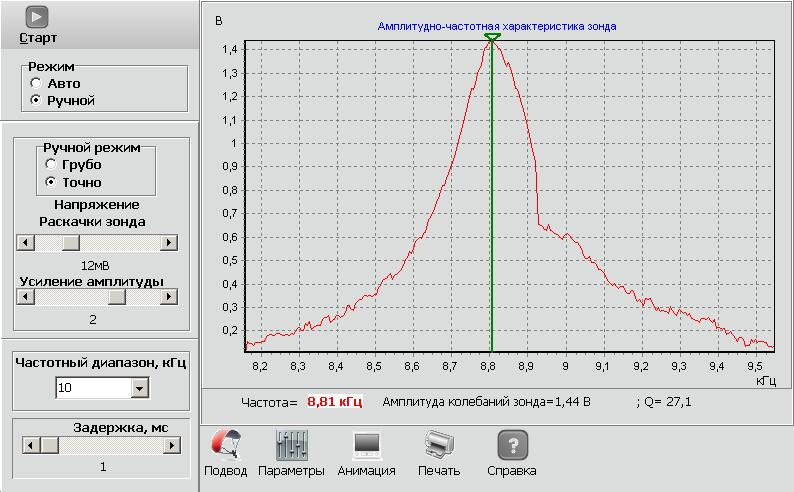
\includegraphics[width=0.7\textwidth]{АЧХ.jpg}
    \caption{Амплитудно-частотная характеристика зонда.}
    \label{fig:ach}
\end{figure}

Полученное значение добротности $Q = 27{,}1$ характерно для колебаний зонда в воздухе и обеспечивает достаточную остроту резонансного пика для работы в бесконтактном режиме. Резонансная частота $f_0 \approx 8{,}8$~кГц была использована в качестве рабочей при последующем сканировании.

Далее был произведён подвод зонда к образцу в режиме \textit{Slow} с чувствительностью обратной связи \textit{Feed Back Loop Gain} $= 3$.






\subsection*{Исследование калибровочной решётки TGT01}

Сканирование решётки TGT01 проводилось со следующими параметрами:
\begin{itemize}
    \item размер области сканирования: $12 \times 12$~мкм$^2$;
    \item разрешение: $600 \times 600$ точек (шаг сканирования $20$~нм);
    \item скорость сканирования: $\approx 2$~сек/строку.
\end{itemize}

Полученное изображение топографии решётки представлено на рис.~\ref{fig:tgt01_topo}.

\begin{figure}[h!]
    \centering
    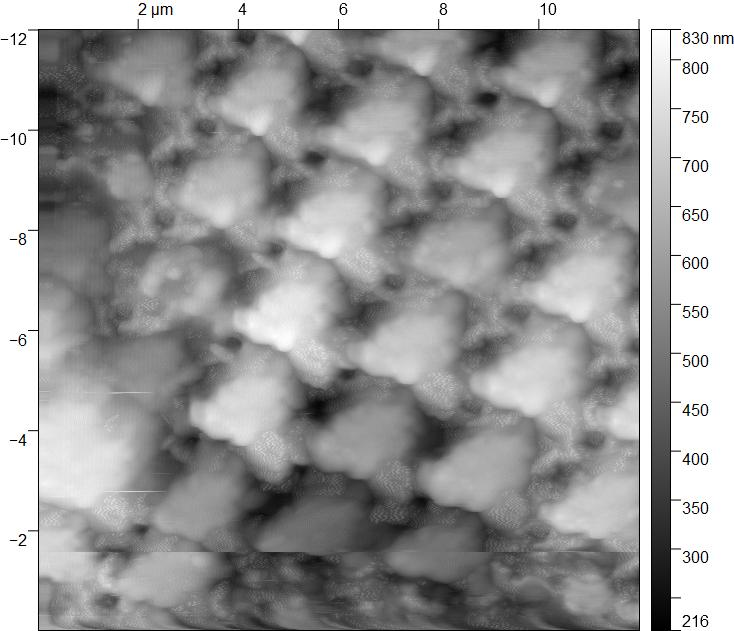
\includegraphics[width=0.6\textwidth]{4.jpg}
    \caption{Топография калибровочной решётки TGT01.}
    \label{fig:tgt01_topo}
\end{figure}

Для количественного анализа рельефа было получено характерное сечение профиля вдоль выступа решётки (рис.~\ref{fig:tgt01_section}).

\begin{figure}[h!]
    \centering
    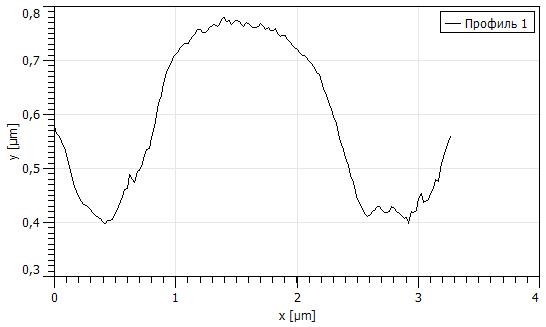
\includegraphics[width=0.7\textwidth]{5.jpg}
    \caption{Сечение профиля решётки TGT01.}
    \label{fig:tgt01_section}
\end{figure}

По сечению были определены следующие геометрические параметры решётки:
\begin{itemize}
    \item период решётки (расстояние между соседними выступами): $a \approx 2,5$~мкм;
    \item высота шапок (глубина провала между выступами): $\Delta Z \approx 0,5$~мкм;
    \item ширина выступа на уровне полувысоты: $d \approx 1,3$~мкм;
    \item угол наклона стенок шапок: $\alpha \approx 20 \text{--} 40^\circ$.
\end{itemize}

Радиус закругления острия зонда был оценён по формуле:
\begin{equation}
    R = \frac{d^2}{2\Delta Z} \approx 1,7~\text{мкм}.
\end{equation}


Измеренный период решётки $a \approx 2{,}5$~мкм превышает паспортное значение $2{,}12$~мкм примерно на $18\,\%$, что указывает на погрешность калибровки пьезосканера или влияние нелинейности. Оценённый радиус закругления зонда $R \approx 1{,}7$~мкм значительно превышает паспортное значение $\sim 10$~нм, что в первую очередь обусловлено износом иглы, а также эффектом уширения профиля: конечный радиус зонда не позволяет ему полностью проникнуть в узкие провалы между выступами, из-за чего измеренная ширина выступа оказывается завышенной.






\subsection*{Исследование фрагмента CD-диска}

Сканирование фрагмента CD-диска проводилось со следующими параметрами:
\begin{itemize}
    \item размер области сканирования: $6 \times 6$~мкм$^2$;
    \item разрешение: $300 \times 300$ точек (шаг сканирования $\approx 20$~нм);
    \item скорость сканирования: $\approx 2$~сек/строку.
\end{itemize}

Полученное изображение топографии поверхности CD-диска представлено на рис.~\ref{fig:cd_topo}.

\begin{figure}[h!]
    \centering
    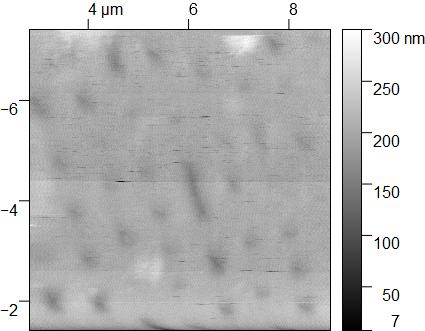
\includegraphics[width=0.6\textwidth]{6.jpg}
    \caption{Топография поверхности CD-диска.}
    \label{fig:cd_topo}
\end{figure}

По сечению профиля дорожек (рис.~\ref{fig:cd_section}) были определены следующие параметры:
\begin{itemize}
    \item глубина питов: $h \approx 40$~нм;
    \item ширина питов: $w \approx 0,45$~мкм;
    \item период дорожек (расстояние между соседними дорожками): $p \approx 0,9$~мкм;
    \item диапазон длин питов: от $0,45$~мкм до $1,25$~мкм.
\end{itemize}

\begin{figure}[h!]
    \centering
    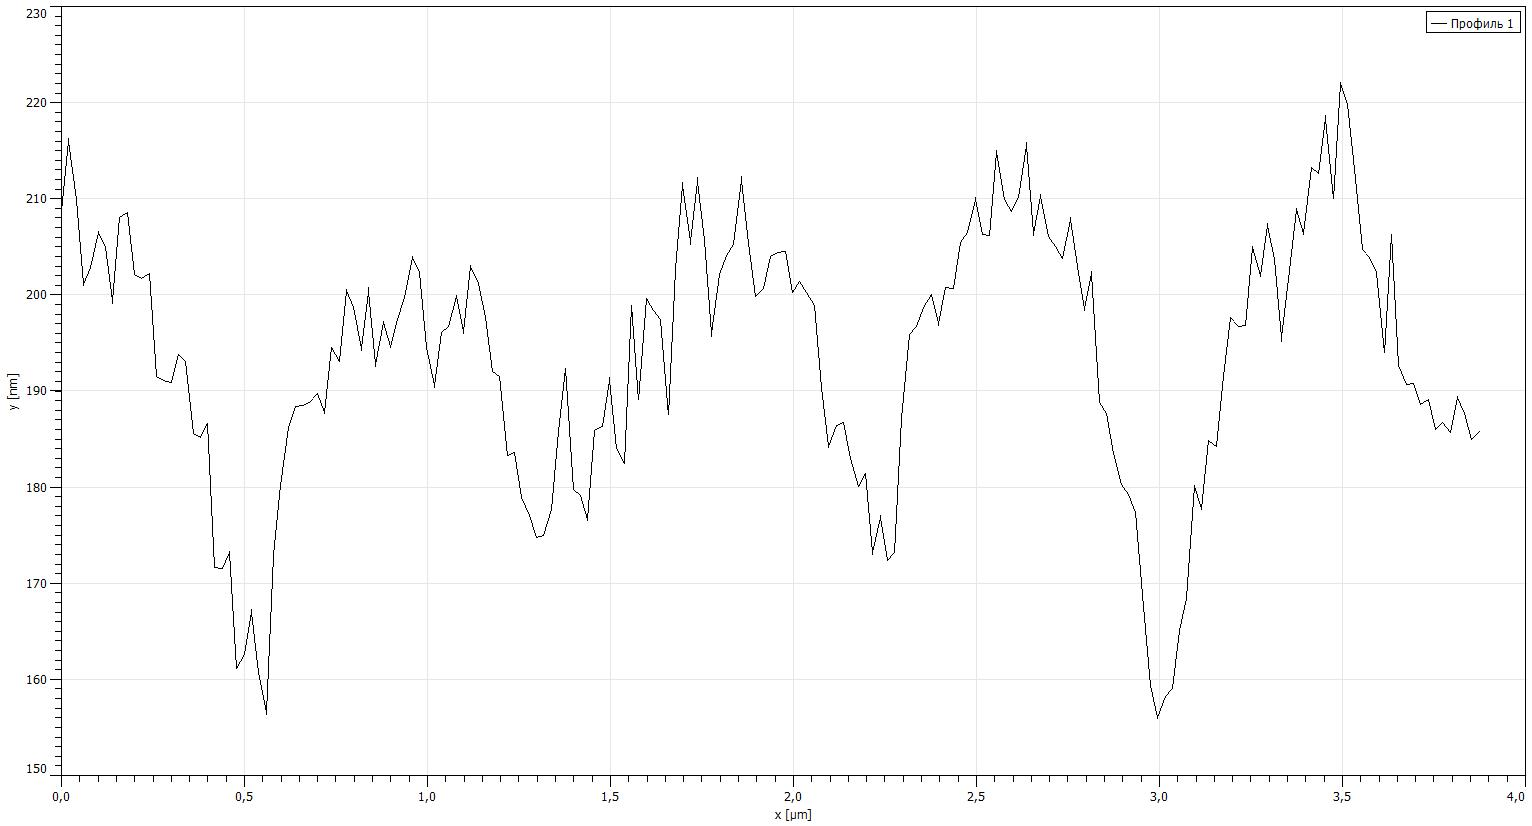
\includegraphics[width=0.7\textwidth]{7.jpg}
    \caption{Сечение профиля дорожек CD-диска.}
    \label{fig:cd_section}
\end{figure}

Измеренный период дорожек $p \approx 0{,}9$~мкм примерно в два раза отличается от стандартного значения для CD-дисков $\approx 1{,}6$~мкм. Столь значительное отклонение, вероятно, связано с погрешностью калибровки пьезосканера по осям $X$ и $Y$. Глубина питов $h \approx 40$~нм соответствует технологическим параметрам записи компакт-дисков (типичная глубина $100\text{--}150$~нм, но с учётом уширения профиля измеренное значение занижено).

\subsection*{Сравнение с паспортными данными}

В таблице~\ref{tab:comparison} приведено сравнение измеренных значений с паспортными данными.

\begin{table}[h!]
\centering
\caption{Сравнение измеренных и паспортных значений}
\label{tab:comparison}
\begin{tabular}{|l|c|c|}
\hline
\textbf{Параметр} & \textbf{Измерено} & \textbf{Паспорт} \\
\hline
Период решётки TGT01, мкм & $2,5$ & $2{,}12$ \\
\hline
Период дорожек CD, мкм & $0,9$ & $\approx 1{,}6$ \\
\hline
\end{tabular}
\end{table}

Расхождения между измеренными и паспортными значениями могут быть обусловлены нелинейностью пьезосканера, гистерезисом, а также конечным радиусом закругления зонда, приводящим к уширению профиля и занижению измеряемых высот.




\subsection*{Спектроскопия}

Спектроскопия в атомно-силовой микроскопии представляет собой метод измерения зависимости амплитуды колебаний зонда от расстояния между зондом и образцом в фиксированной точке поверхности. Данный метод позволяет исследовать характер сил взаимодействия зонда с поверхностью и определить оптимальные параметры для работы в бесконтактном режиме.

Измерения проводились в режиме \textit{Spectroscopy} со следующими параметрами:
\begin{itemize}
    \item начальная точка: $Z_0 = -300$~нм;
    \item конечная точка: $Z_{end} = 100$~нм;
    \item количество точек: $200$;
    \item шаг сканирования: $\approx 2{,}01$~нм;
    \item задержка: $1$~мс.
\end{itemize}

Зависимость амплитуды колебаний зонда от расстояния зонд--образец, полученная в точке 3, представлена на рис.~\ref{fig:spectroscopy_main}. На графике отображены две кривые: красная соответствует подводу зонда к поверхности, синяя --- отводу.

\begin{figure}[h!]
    \centering
    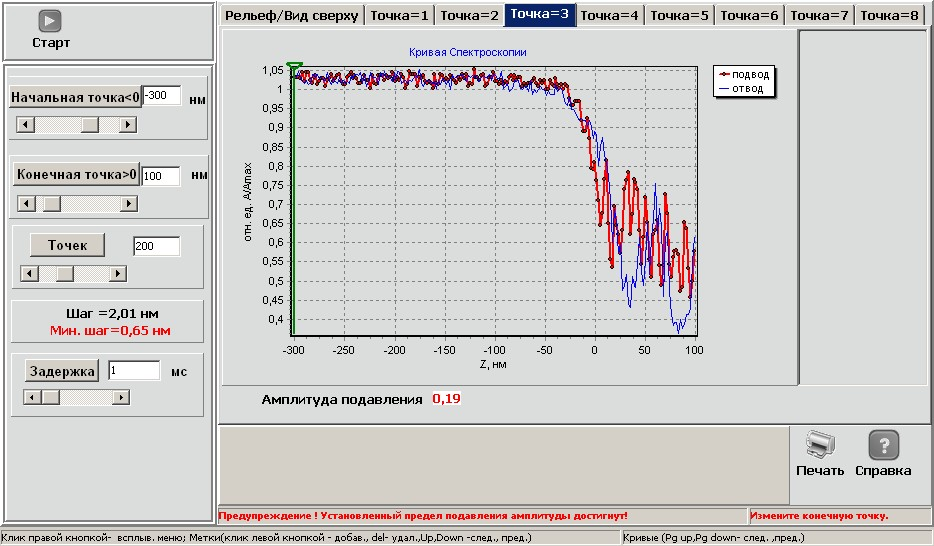
\includegraphics[width=0.8\textwidth]{10.jpg}
    \caption{Зависимость амплитуды колебаний зонда от расстояния зонд--образец (точка 3). Красная кривая --- подвод, синяя --- отвод.}
    \label{fig:spectroscopy_main}
\end{figure}

На полученной кривой выделяются три характерные области:

\begin{enumerate}
    \item \textbf{Область свободных колебаний} ($Z$ от $-300$ до $-50$~нм). Амплитуда колебаний постоянна и максимальна ($A/A_{max} \approx 1{,}0$). В этой области зонд находится далеко от поверхности, силы взаимодействия пренебрежимо малы, и зонд колеблется на резонансной частоте с максимальной амплитудой.
    
    \item \textbf{Область взаимодействия} ($Z$ от $-50$ до $0$~нм). При приближении зонда к поверхности амплитуда начинает плавно уменьшаться. Это связано с действием дальнодействующих сил притяжения (ван-дер-ваальсовых и капиллярных), которые изменяют эффективную жёсткость колебательной системы и смещают резонансную частоту.
    
    \item \textbf{Область контакта} ($Z > 0$~нм). Наблюдается резкое падение амплитуды с сильными флуктуациями. Зонд переходит в режим отталкивания, происходит ``захват'' зонда поверхностью. Флуктуации амплитуды связаны с нестабильностью контакта и возможным проскальзыванием зонда по поверхности.
\end{enumerate}

Особый интерес представляет расхождение между кривыми подвода и отвода в области контакта ($Z > 0$~нм), известное как \textbf{гистерезис}. Это явление обусловлено капиллярными силами: при подводе зонд ``проваливается'' в жидкий мостик, образующийся из адсорбированной воды на гидрофильной поверхности, а при отводе --- ``вырывается'' из него. Для преодоления капиллярных сил при отводе требуется большее расстояние, что и приводит к наблюдаемому расхождению кривых.

Для сравнения на рис.~\ref{fig:spectroscopy_all} представлены спектроскопические кривые, полученные в четырёх различных точках поверхности CD-диска. Все кривые демонстрируют схожую форму, что подтверждает воспроизводимость результатов.

\begin{figure}[h!]
    \centering
    \begin{tabular}{cc}
        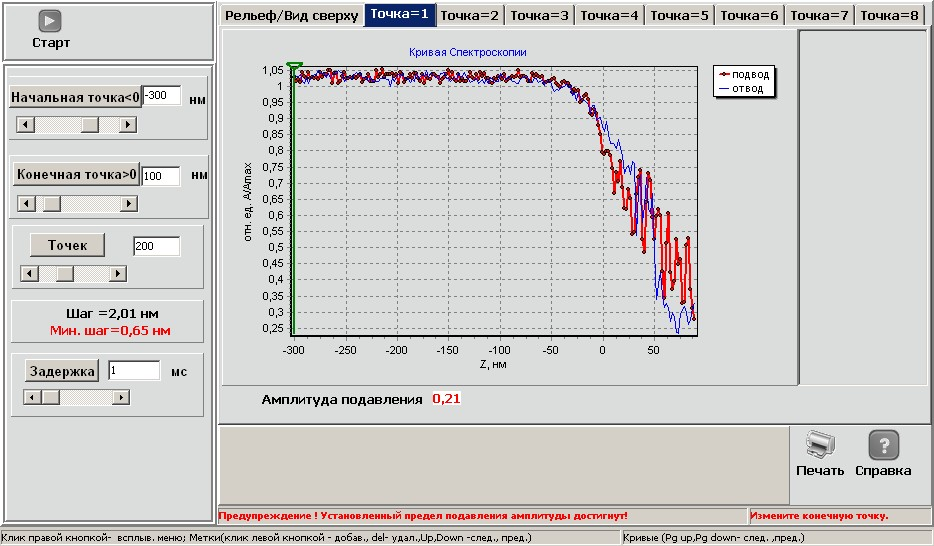
\includegraphics[width=0.45\textwidth]{8.jpg} &
        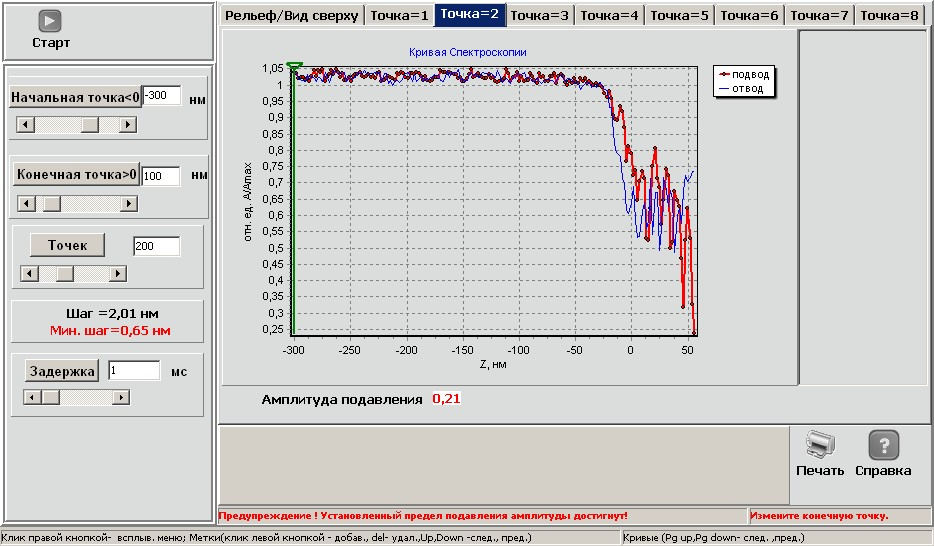
\includegraphics[width=0.45\textwidth]{9.jpg} \\
        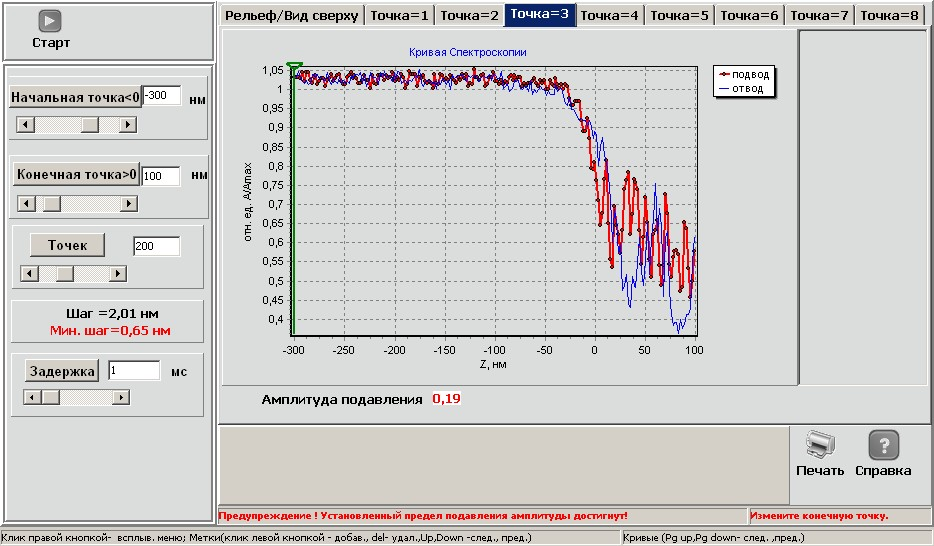
\includegraphics[width=0.45\textwidth]{10.jpg} &
        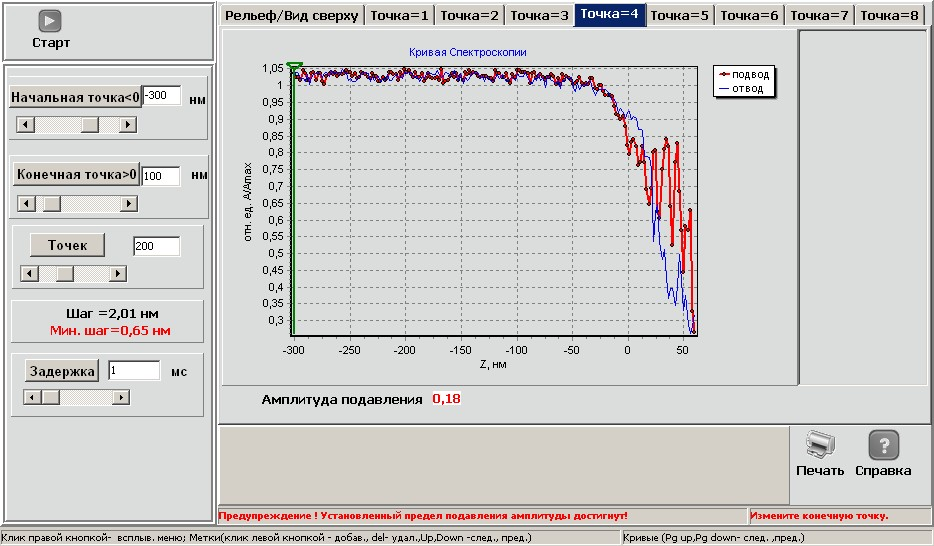
\includegraphics[width=0.45\textwidth]{11.jpg}
    \end{tabular}
    \caption{Спектроскопические кривые в четырёх точках поверхности CD-диска.}
    \label{fig:spectroscopy_all}
\end{figure}

Форма полученных спектроскопических кривых соответствует теоретическим представлениям о поведении зонда в бесконтактном режиме. Плавное падение амплитуды при $Z \approx -50$~нм свидетельствует о начале действия дальнодействующих сил притяжения. Резкий скачок при $Z \approx 0$~нм соответствует переходу в контактный режим. Наблюдаемый гистерезис между кривыми подвода и отвода обусловлен капиллярными силами, характерными для измерений на воздухе с гидрофильными поверхностями. Полученные данные подтверждают корректность выбора параметров для работы в бесконтактном режиме.







\section*{Выводы}

В ходе выполнения лабораторной работы были изучены физические принципы функционирования атомно-силового микроскопа и проведены измерения на сканирующем зондовом микроскопе \textit{NanoEducator} в бесконтактном режиме.

Была настроена резонансная частота зонда ($f_0 \approx 8{,}8$~кГц) и определена добротность колебательной системы ($Q = 27{,}1$), что обеспечило корректную работу в бесконтактном режиме.

По результатам сканирования калибровочной решётки TGT01 были определены её геометрические параметры: период решётки $a \approx 2{,}5$~мкм, высота шапок $\Delta Z \approx 0{,}5$~мкм, угол наклона стенок $\alpha \approx 20\text{--}40^\circ$. Оценён радиус закругления острия зонда: $R \approx 1{,}7$~мкм.

При исследовании фрагмента CD-диска получены следующие параметры: глубина питов $h \approx 40$~нм, ширина питов $w \approx 0{,}45$~мкм, период дорожек $p \approx 0{,}9$~мкм, диапазон длин питов от $0{,}45$ до $1{,}25$~мкм.

В режиме спектроскопии снята зависимость амплитуды колебаний зонда от расстояния зонд--образец. На кривой выделены три характерные области: свободных колебаний, взаимодействия и контакта. Наблюдаемый гистерезис между кривыми подвода и отвода обусловлен капиллярными силами.

Измеренные значения периода решётки TGT01 и периода дорожек CD-диска отличаются от паспортных данных на $18\,\%$ и $44\,\%$ соответственно. Основные источники погрешностей:
\begin{itemize}
    \item нелинейность и гистерезис пьезосканера (до $10\text{--}20\,\%$);
    \item температурный дрейф пьезокерамики;
    \item эффект уширения профиля из-за конечного радиуса закругления зонда ($R \approx 1{,}7$~мкм), приводящий к занижению измеряемых высот и завышению ширин выступов;
    \item износ (затупление) острия зонда в процессе эксплуатации, что дополнительно увеличивает эффективный радиус кривизны и усугубляет искажение геометрии рельефа.
\end{itemize}

Полученные результаты подтверждают возможность применения АСМ для исследования топографии поверхности с нанометровым разрешением, а также демонстрируют влияние инструментальных погрешностей на точность измерений.


\end{document}